%! Author = Filippo Vissani
%! Date = 08/02/24
% !TeX root = ../thesis-main.tex

%----------------------------------------------------------------------------------------
\chapter{Design}
\label{chap:design}
%----------------------------------------------------------------------------------------

\section{Architecture}

As mentioned in \Cref{subsection:collektive-architecture}, Collektive consists of three main modules: \texttt{dsl}, \texttt{compiler-plugin} and \texttt{alchemist-incarnation-collektive}.\\ \texttt{alchemist-incarnation-collektive} is responsible for enabling the integration of Collektive simulations into Alchemist. The \texttt{compiler-plugin} takes care of visiting the abstract syntax tree of the aggregate expression and modifying the function call stack to correctly align the devices that execute the aggregate program. The \texttt{dsl} module defines the following components:
\begin{itemize}
    \item \texttt{aggregate}: deals with defining the context related to a device, the semantics of aggregate constructs, and the data structures necessary for path definition and device alignment;
    \item \texttt{field}: Contains the definition of computational field and the related functionalities for manipulating the latter;
    \item \texttt{state}: defines the association between the paths and the results of their evaluations;
    \item \texttt{path}: Defines the data structures necessary to represent the abstract syntax tree relating to the aggregate expression;
    \item \texttt{networking}: defines the data structures necessary for distributed device communication.
\end{itemize}

Given the solutions proposed in \Cref{subsection:integration-solutions-identified}, in both cases, it is necessary to review some of the entities present in Collektive so that it is possible to detect and react to their changes. Regardless of the detailed solution chosen, given that the Collektive design allows it, it is possible to introduce the necessary functionalities as an extension of the current ones. The proposed architecture is shown in \Cref{fig:collektive-prm-architecture}, the components in gray are part of the current Collektive architecture, and those in orange introduce the entities that enable reactive aggregate programming. The component \texttt{reactive} extends \texttt{aggregate} to introduce a reactive version of the entities described above and \texttt{network} to allow reactive distributed communication between devices. The component \texttt{flow.extensions} is used to simplify some operations for combining and mapping flows. According to this design choice, the other modules in the project (\texttt{compiler-plugin} and \texttt{alchemist-incarnation-collektive}) are not altered; consequently, the reactive model introduced continues to make use of the compiler plugin for the definition of the paths.

\begin{figure}
    \centering
    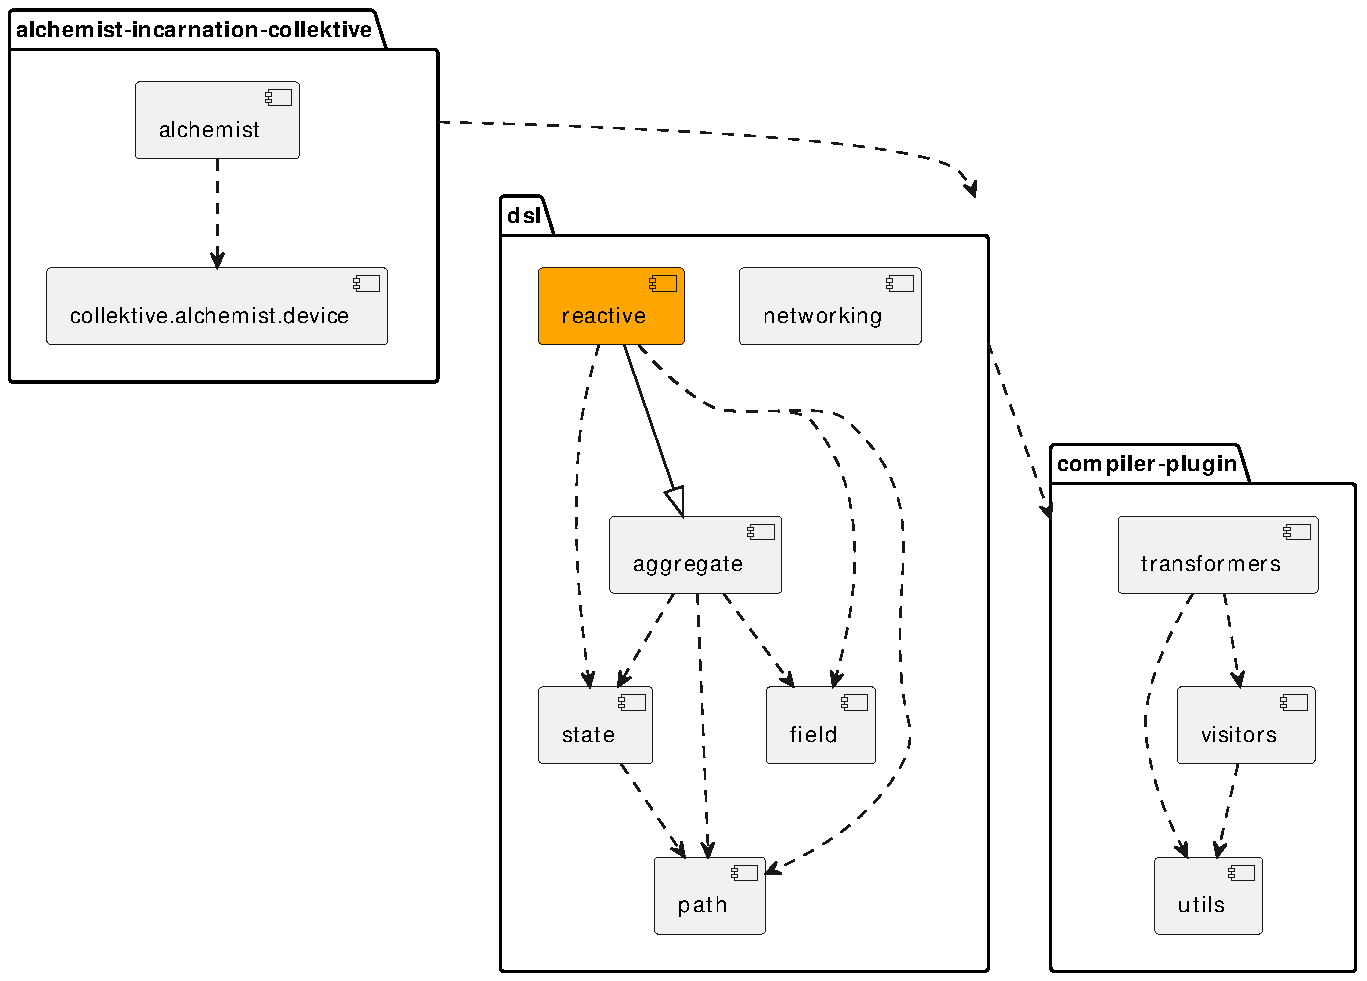
\includegraphics[width=\linewidth]{figures/collektive-prm-architecture.pdf}
    \caption{Architecture of the purely reactive model proposed. The gray-colored components are part of the original Collektive architecture, while the orange-colored components are used to introduce the reactive paradigm.}
    \label{fig:collektive-prm-architecture}
\end{figure}

\section{Detailed Design}

\subsection{Purely Reactive Model}

\begin{figure}
    \centering
    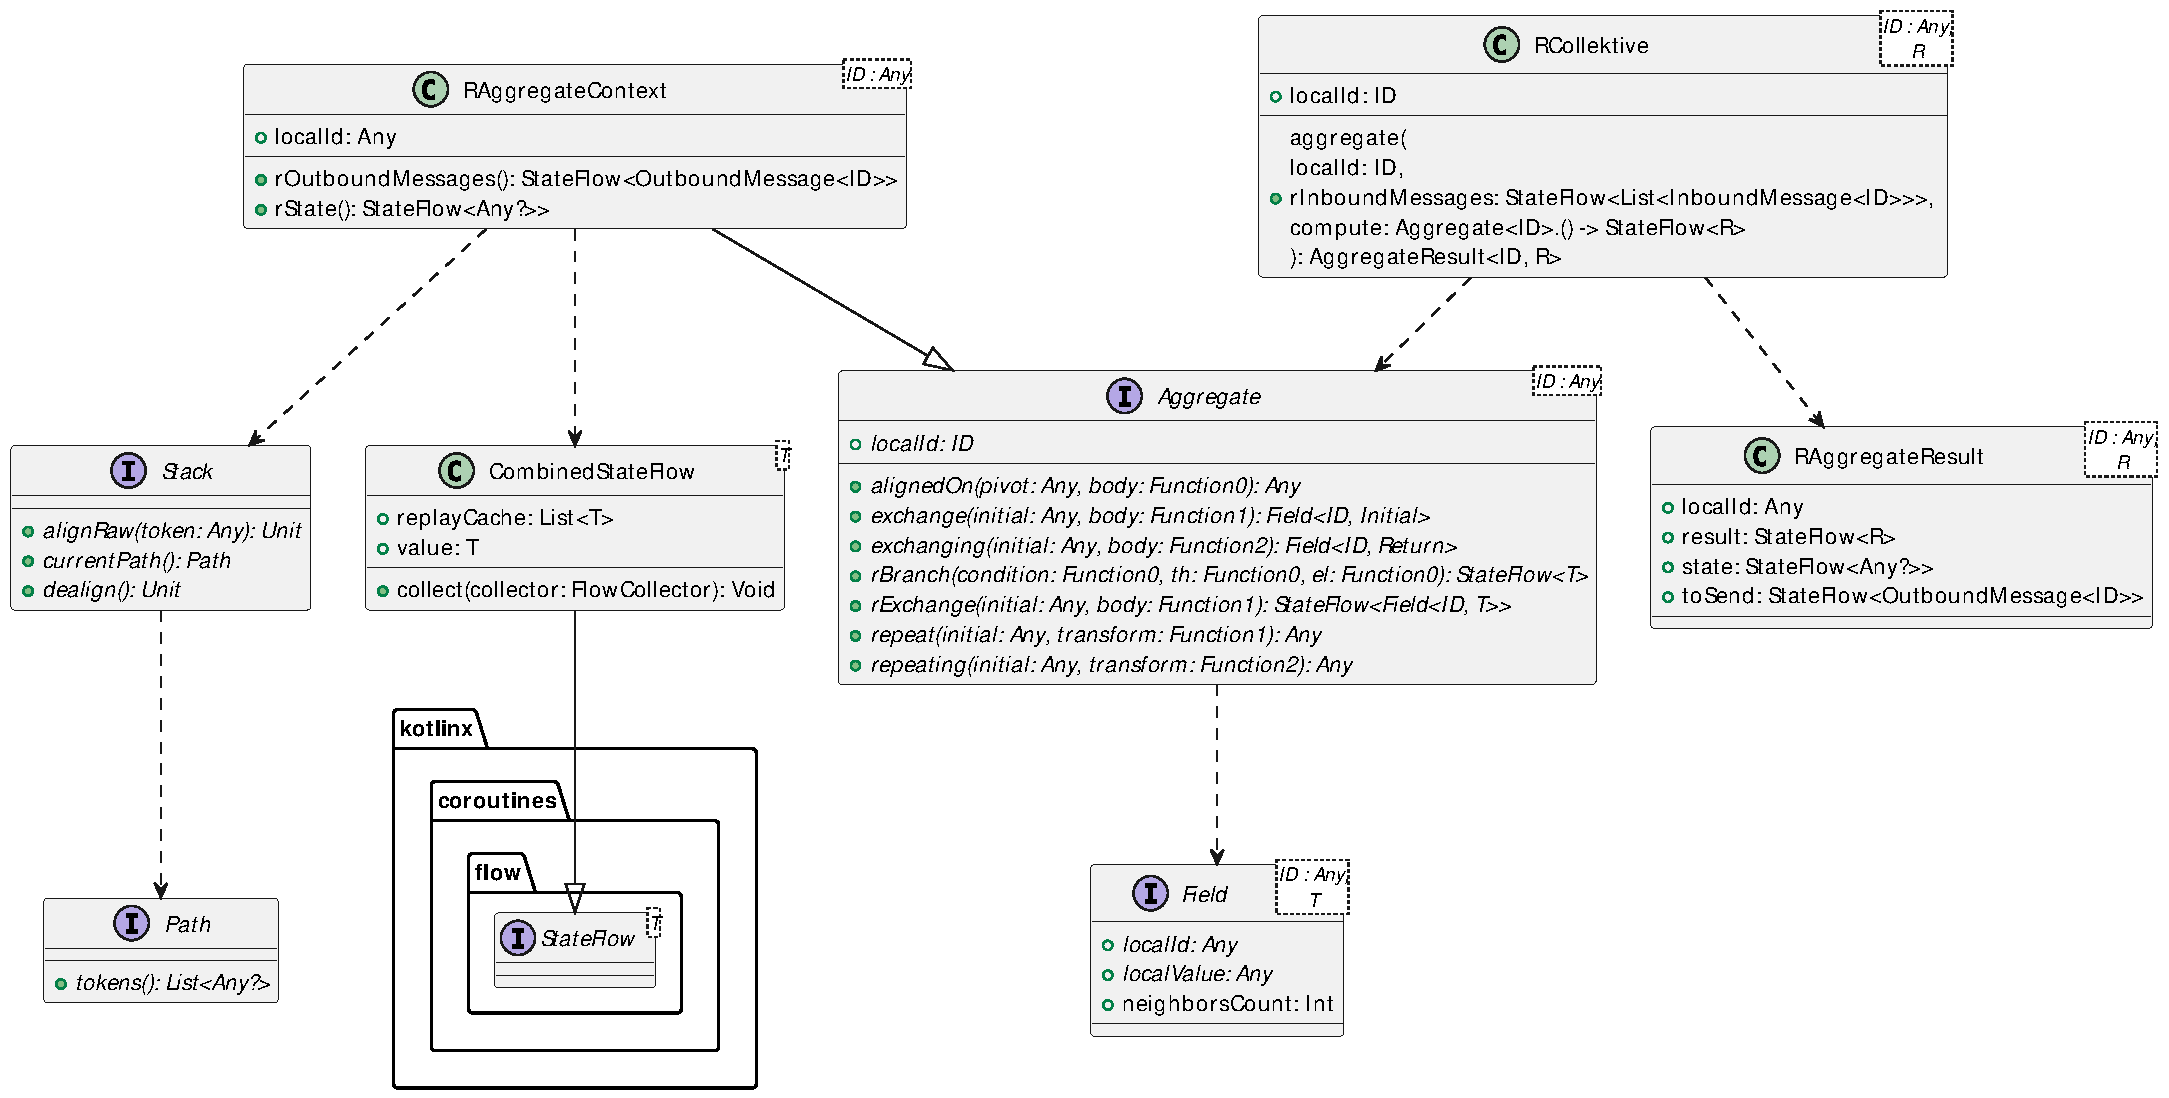
\includegraphics[width=\linewidth]{figures/collektive-prm-design.pdf}
    \caption{Detailed design of the purely reactive model proposed.}
    \label{fig:collektive-prm-design}
\end{figure}

\subsection{Model with Reactive Messages and Sensors}

\begin{figure}
    \centering
    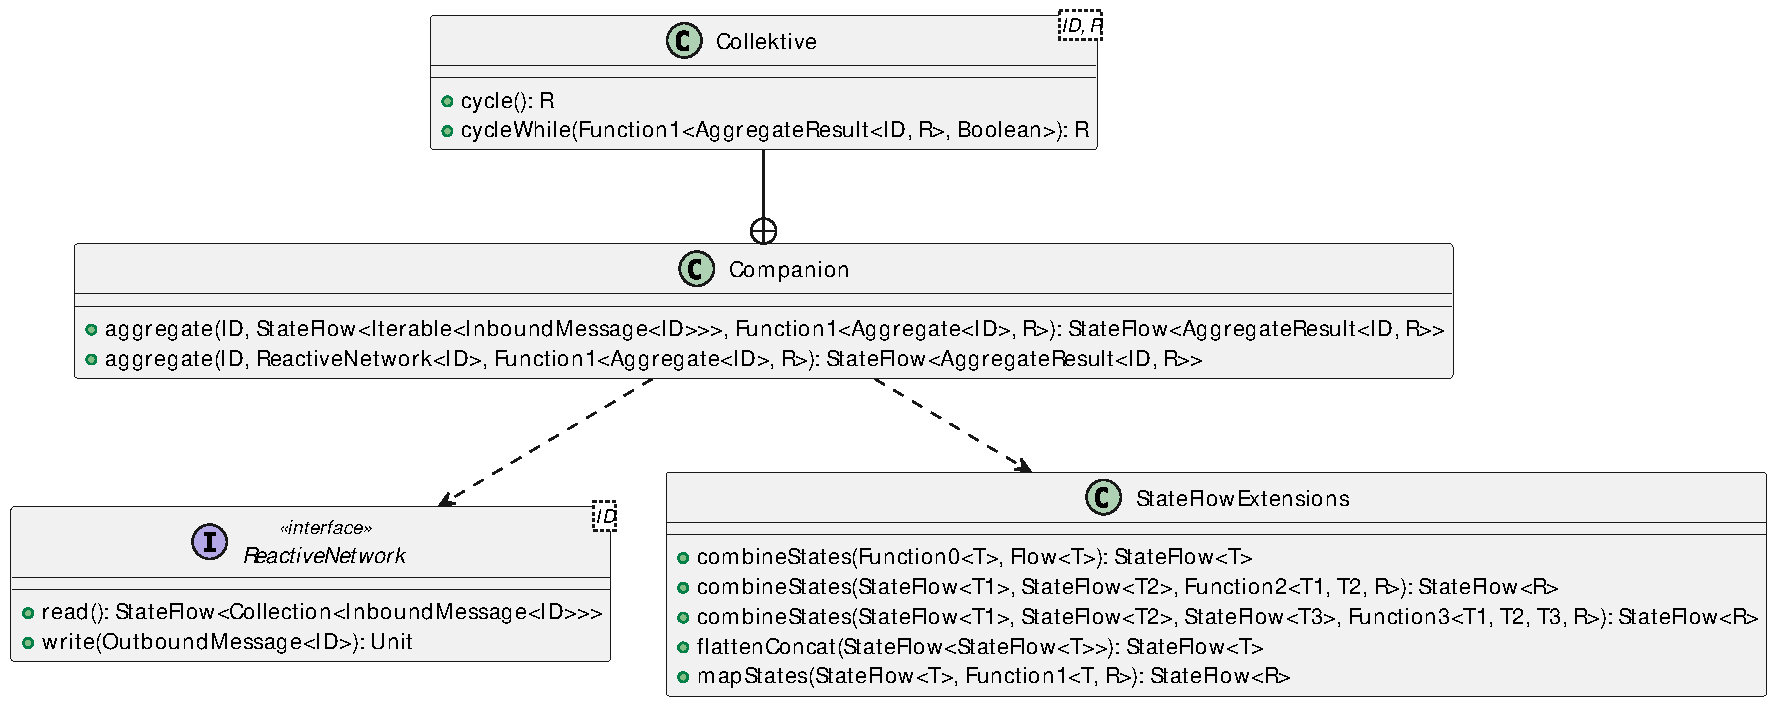
\includegraphics[width=\linewidth]{figures/collektive-rmsm-design.pdf}
    \caption{Detailed design of the model with reactive messages and sensors.}
    \label{fig:collektive-rmsm-design}
\end{figure}
